\documentclass[a4paper,10pt]{article}

\usepackage{geometry}

\usepackage[utf8x]{inputenc}
\usepackage[bookmarks,colorlinks=false,pdfborder={0 0 0}]{hyperref}
\hypersetup{pdftitle={Unternehmensorientierung - Geschäftsidee: gamergeld.de}}
\usepackage{url}
\usepackage[ngerman]{babel}
\usepackage{graphicx}
\usepackage{listings}

\parindent 0pt
\parskip 10pt

\title{Unternehmensorientierung - Geschäftsidee: gamergeld.de}
\author{Erik Andresen \and Andreas Basener \and Jan Depke \and Andreas Krohn \and Benjamin Vetter}

\begin{document}

\maketitle

\section{Geschäftsidee}
\emph{Zentralisierte Zahlungsabwicklung für Browsergames/Free-to-Play Games}

Kooperation mit Gameherstellern

Gamehersteller sollten/werden mit uns kooperieren, weil
\begin{itemize}
  \item weniger Implentierungsaufwand (vor allem: neue Spiele)
  \item Verlinkung von unserer Seite - damit: Bekanntheitsgewinn
\end{itemize}

Wir bieten eine API für Gamehersteller an.
Die Wechselkurse zur jeweiligen Gamewährung werden per API übergeben.

Spieler wird z.B. beim Kauf eines Items auf gamergeld.de redirected und zahlt dort den geforderten Betrag bzw. belastet sein Konto.
Zahlung über Paypal, clickandbuy, giropay, Kreditkarte, Bankeinzug, sofortüberweisung, Moneybookers, Bitcoins, Prepaid, ..

\subsection{Risiken}
\begin{itemize}
  \item Zahlungsausfall
  \item Klar als Vermittler und nicht als Anbieter der Items kennzeichnen (Regress..)
\end{itemize}

\section{Tragfähigkeit}\label{labelTragfaehigkeit}

\subsection{Marktuntersuchung}\label{labelMarktuntersuchung}
Depke
\begin{itemize}
  \item Gibt es ähnliche Anbieter?
  \item Wie hoch sind die zu zahlenden Preise bei Browsergames?
  \item Wieviele (zahlende) User in Browsergames?
\end{itemize}

\subsection{Technische Machbarkeit}\label{labelTechMach}

Um unsere Dienstleistung für Gamehersteller anbieten zu können verwenden wir
die individuellen APIs der spezifischen Zahlungsanbieter und bieten
unsererseits eine einheitliche API für die Gamehersteller an. Alle in diesem
Dokument genannten Zahlungsanbieter verfügen über derartige APIs, sodass diese
problemlos von uns integriert werden können. Jeder Gamehersteller kann
Zahlungstransaktionen über unsere abstrahierte API durchführen und dadurch alle
von uns verwendeten Zahlungsanbieter unterstützen. 

\subsubsection{API}
Um die Verwendung unserer API möglichst einfach zu gestalten und die API
unsererseits nicht in allen gängigen Programmiersprachen implementieren zu
müssen, bietet sich die Verwendung gängiger Protokolle an, um die API
programmiersprachen- und plattformunabhängig zu gestalten. Die API werden wir
daher REST-basiert implementieren. Durch den HTTP-Unterbau von REST kann die
API in allen gängigen Programmiersprachen problemlos und ohne zusätzlichen
Aufwand unsererseits verwendet werden. Der grobe Protokollablauf für eine
einzelne Transaktion sieht bspw. wie folgt aus:

\begin{enumerate}
  \item Der Gamehersteller erstellt eine neue Transaktion für das zuvor im Account
    erstellte Game und über einen bestimmten Betrag
  \item Die Response teilt die Transaktionskennung mit
  \item Der Gamer wird zu gamergeld.de weitergeleitet oder alternativ wird gamergeld.de
    innerhalb eines iFrames angezeigt um die Transaktion innerhalb des Spiels durchzuführen
  \item Auswahl der Zahlungsart und ggf. des Zahlungsanbieters durch den Gamer, ggf. Login
  \item Durchführung der Zahlung
  \item Benachrichtigung des Zahlungsanbieters über Erfolg/Misserfolg der Transaktion,
    bspw. über eine vom Hersteller spezifizierte URL und mit Transaktionskennung
  \item Damit ist das Protokoll abgeschlossen
\end{enumerate}

\subsubsection{Infrastruktur}
Um auch auf Wachstum über die in diesem Dokument spezifizierten Erwartungen
hinaus eingestellt zu sein und eine grundsätzlich leicht skalierbare
Architektur bei planbaren Kosten zu realisieren, bietet sich die Verwendung von
Cloud-Angeboten an. Indes muss die Verfügbarkeit der verwendenten Infrastruktur
überdurchschnittlich sein, da eine Nicht-Verfügbarkeit von gamergeld.de einen
Zahlungsausfall seitens unserer Kunden nach sich zieht.

Dabei kommen Cloud-Lösungen bzgl. der verwendeten Server-, Storage- und
Datenbank-Infrastruktur, ebenso wie Load-Balancer-Lösungen in Frage.
Storage-Lösungen sind dabei jedoch von untergeordnetem Interesse, da diese nur
bzgl. Content-Delivery (CDN) für die statischen Mediendaten, die in die Website
eingebettet sind, in Frage kommen. Große und umfangreiche Mediendaten werden
hingegen von gamergeld.de nicht vorgehalten. Beispiele für derartige
Cloud-Lösungen sind bspw. die Angebote von Amazon \cite{Amazon} und Rackspace
\cite{Rackspace}. Die Kosten eines durchschnittlichen Cloud-Servers (EC2) von
Amazon belaufen sich derzeit bei rund \$227.50 jährlich \cite{Amazon}. Amazon
gibt die Verfügbarkeit ihrer Services mit 99.95\% an \cite{Amazon}. Dennoch
müssen, zwecks Redundanz und Fehlertoleranz, mehrere Server in vorzugsweise
mehreren Rechenzentren vorgehalten werden, sodass die Kosten dafür zu Beginn
bei \$800-1500 jährlich liegen. Die exakte Anzahl zu verwendenden Servern ist
abhängig vom Traffic und Transaktionsvolumen. Unsere Architektur ist auch
kurzfristig skalierbar.

Bzgl. der Datenbanken verwenden wir keine zusätzlichen Cloud-basierten
Datenbanken wie bspw. Amazon RDS, sondern verwenden MySQL- und
MongoDB-Datenbanken, die sich auf den von uns betriebenen Servern befinden.
Das hat den zusätzlichen Vorteil, dass bspw. Kundendaten ausschließlich auf
Systemen gespeichert sind, die von uns administriert werden. Die
MySQL-Datenbanken werden für Account- und andere Kundendaten verwendet,
betreiben eine Master-Slave und/oder Master-Master Replikation und sind daher
bzgl. der Read-Anweisungen gut skalierbar. Bzgl. der Write-Anweisungen wird
jedoch nur moderate Skalierbarkeit erreicht. Häufige Änderungen an Account- und
Kundendaten sind jedoch idR. nicht zu erwarten, sodass hierbei keine Probleme
entstehen. Für die Speicherung von Transkationsdaten sind die MySQL-Systeme bei
hohen Transaktionsvolumina jedoch, ohne umfangreiche Maßnahmen, nur bedingt
geeignet. Daher vewenden wir für die Transaktionensdaten MongoDB-Datenbanken,
ebenfalls mit Master-Slave und Master-Master Replikation, da NoSQL-Datenbanken
bzgl. der Write-Anweisungen einfacher zu skalieren sind\footnote{Bspw. da
Sharding bei denormalisierten Datenbanken deutlich einfacher zu realisieren
ist.}.

\subsubsection{Sicherheit}
Insider-Angriffe seitens des Cloud-Anbieters können wir nur z.T.
berücksichtigen. Jedoch dürfen Account-, Kunden-, Kreditkarten- und
Transaktionsdaten serverseitig ausschließlich auf Systemen gespeichert werden,
die von uns administriert werden. Da wir keine zusätzlichen Cloud-basierten
Datenbanken verwenden ist dies jedoch gewährleistet.

Da gamergeld.de u.a. Kreditkartendaten entgegennimmt und speichert, gelten für
die verwendeten System besonders hohe Sicherheitsanforderungen und
Schutzkategorien. Unter anderem müssen unsere Systeme die PCI-Compliance Tests
bestehen \cite{PCI}, die für alle Unternehmen und Systeme, die
Kreditkartendaten verarbeiten, gelten. Das ist mit entsprechenden
Schutzmaßnahmen, als auch mit Kosten für die PCI-Compliance-Tests verbunden.
Die Kosten für derartige Tests müssen idR. vierteljährlich durchgeführt werden,
sind abhängig von der Anzahl verwendeter IP-Adressen als auch von den
Transaktionvolumina. Pro IP-Adresse und Quartal belaufen sich die Kosten pro
IP-Adresse daher bei ca. 220 EUR \cite{PCI:Costs}, also ca. 4000 EUR jährlich
für das beschriebene Setup.

Bzgl. der Serversicherheit werden ausserdem typische Best-Practices, wie
Policies und Patch-Zyklen, Firewalls, verschlüsselte Kommunikation (SSH, SSL),
Authentifikation, etc. verwendet.


\newpage
\subsection{Finanzierung und wirtschaftliche Machbarkeit}\label{labelWirtMach}
%Gesamtplan 3-5 Jahre

Für die Berechnung unserer Finanzierung und der wirtschaftlichen Machbarkeit werden folgende Annahmen getroffen:

Als einzelne Kostenpositionen erwarten wir folgende Posten:
\begin{itemize}
\item Fixkosten
 \begin{itemize}
\item Serverkosten
\item Personalkosten
\item Büromiete
\item Kredittilgungen
 \end{itemize}
\item variable Kosten
\begin{itemize}
\item Marketingkosten
\item Entwicklungskosten
\item Transaktionsgebühren
\item Kreditzinsen
\item Bürobedarf/Sonstiges
\end{itemize}
\end{itemize}

Die Kosten für die Server ergeben sich aus den Betrachtungen im Kapitel \ref{labelTechMach}. Die vermuteten Kosten für das Büro sind dem aktuellen Hamburger Mietspiegel entnommen. Die Personalkosten verteilen sich auf die fünf Mitglieder dieses Unternehmens. Der für die Finanzierung benötigte Kredit erzeugt mit Zinsen und Tilgungen weitere Kosten.\\
Um die Kunden gewinnen zu können entstehen uns Kosten, die unter Marketingkosten zusammengefasst werden. Diese werden im laufe der Zeit abnehmen, wenn unser Bekanntheitsgrad ansteigt.\\
Die benötigte Software zur Zahlungsabwicklung mit den Kunden wird von uns selber entwickelt. Die veranschlagten Kosten sind unter dem Punkt Entwicklungskosten berücksichtigt. Die Entwicklungskosten werden im Laufe der Zeit abnehmen und werden um Wartungskosten ergänzt.\\
Weitere Kosten sind im Punkt Bürobedarf/Sonstiges zusammengefasst und können nur grob geschätzt werden.

Wie in Kapitel \ref{labelMarktuntersuchung} beschrieben, existieren diverse Spieleanbieter am Markt, die jeweils einen hohen Jahresumsatz erzielen. \\
Wir wollen mit unsren Kunden eine langfristige Geschäftsbeziehung eingehen. Wir setzen dabei darauf, dass wir nur einige wenige Kunden benötigen. Durch diese wenigen Kunden können wir aber hohe Umsätze erzielen.

Die Strategie, die wir bei der Kundengewinnung verfolgen, ist, dass wir zu Anfang mit einem Kunden starten und dann nach und nach weitere Kunden gewinnen. 

\subsubsection*{Gewinn und Verlustrechnung}
%24 auf monatlicher Basis, danach jährlich

\begin{figure}[htbp]
	\centering
	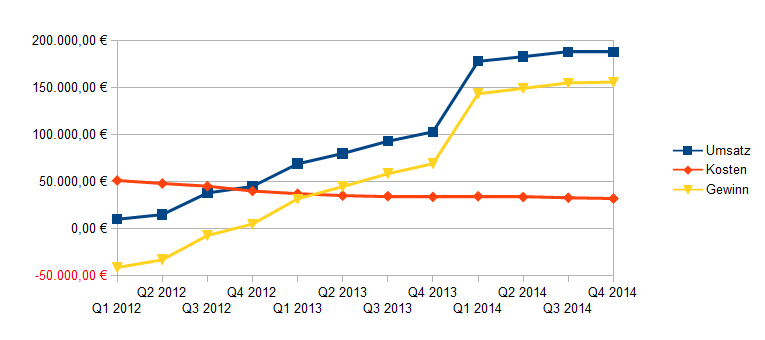
\includegraphics[width=1\textwidth]{GuV.png} 
	\caption{GuV}
	\label{picGuV}
\end{figure}

Die zu erwartenden Kosten betragen pro Quartal im Schnitt ca{.} 40.000,- Euro in den ersten 3 Jahren. Um Kostendecken arbeiten zu können müssen wir diesen Betrag über die Transaktionsgebühren wieder einholen. Wenn wir einen Anteil von 5\% an den Geldtransaktionen für uns einbehalten, dann müssen pro Quartal 800.000,- Euro bei den Kunden umgesetzt werden. 

Wie in Kapitel \ref{labelMarktuntersuchung} dargestellt, sind das sehr vorsichtige Berechnungen. Es ist davon auszugehen, dass der Umsatz bei den Kunden höher liegen wird. Dadurch können wir einerseits unsere eigenen Umsätze erhöhen und Gewinne einfahren, andererseits aber auch den prozentualen an den Kundenumsätzen verringern, was uns einen Vorteil bei Vertragsverhandlungen mit den Kunden einbringt.

\subsubsection*{Liquiditätsrechnung}
%24 auf monatlicher Basis, danach jährlich
\begin{figure}[htbp]
	\centering
	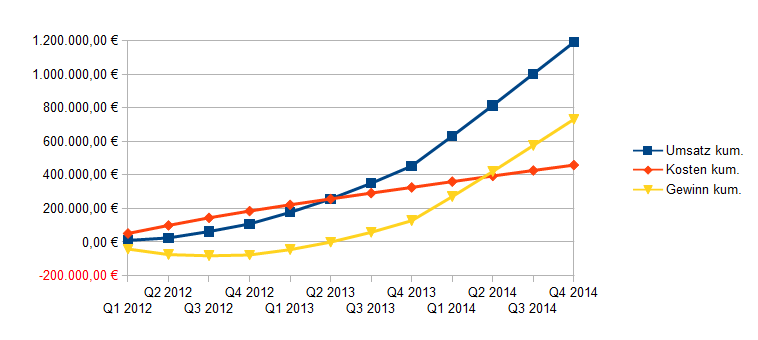
\includegraphics[width=1\textwidth]{GuVkummuliert.png}
	\caption{GuV kumuliert}
	\label{picGuVkum}
\end{figure}

Der Break-Even Punkt wird im vierten Quartal 2012 überschritten. Bis zum vorhergehenden Quartal addieren sich die Verluste auf ca{.} 82.000,- Euro (s. Abbildung \ref{picGuVkum}). Dieser Betrag wird mindestens benötigt, um die zu erwartenden Kosten zu decken.\\
Die Deckung der Kosten wird durch eine Bankfinanzierung geschehen. Dazu nehmen wir einen Kredit in Höhe von 90.000,- Euro mit einer Laufzeit von 4 Jahren und einem Zinssatz in Höhe von 5\%. Die monatlichen Tilgungsraten betragen 1.875,- Euro. Die Kosten sind in den übrigen Berechnungen bereits enthalten.



\section{Relevante Daten}\label{labelRelDaten}
Andresen

\section{Projektplan/Geschäftsplan}\label{labelGeschaeftsplan}
Krohn
% Ergebnisse der Validierung zusammenfassen...

\bibliographystyle{plain}
\bibliography{protokoll}

\end{document}
